\clearpage
\section{Inclusive Charge Current event selection}
\label{sec:InclusiveSelection}

The muon neutrino beam produced at J-PARC passes through the 
off-axis ND280 detector. 
These neutrinos can have Charged Current (CC) 
or Neutral Current interactions with the detector material. 
The CC interactions are expected to produce a $\mu^-$ track
and these $\mu^-$ tracks usually contain  most of 
the momentum from the incident neutrino.
Therefore we search for the highest momentum negative track 
which simplifies the identification and tagging of  
a CC interaction event candidate. %\\
%It is important to note that 
We note that 
the beam spill delivered by J-PARC 
to the experiment has a sub-structure of bunches which are 
separated by beam dead-time. 
All analyses described in this document were done 
at the bunch level instead of the ND280-DAQ event level (Spill level).\\
hjbvjvjv

The selection procedure includes 
the three main information levels 
and 
%. The selection flow 
is listed below:
%includes three steps that correspond
%to the three information levels, (that follow each other) 
%which are
\begin{itemize}
\item 
Beam and Data Quality information:\\
Each Spill is checked to have
\begin{itemize}
\item 
Beam Data flag: `GoodSpillFlag' set to the value of one
\item
Data Quality flag: `ND280OffFlag' equal to zero
\end{itemize}
\item 
Individual global track information: \\
Each track in a good spill is required to have 
\begin{itemize}
\item
The `Status' flag not set to zero
\item
The `FrontMomentum' property %!= 10,000 
not equal to the default value of 10,000
\item
 Its start position (`FrontPosition') 
inside the analysis~\p0d~Fiducial~Volume 
\item
Measured information from TPC1 sub-detector
\end{itemize}

\item 
Bunch time window information: \\
At this stage the tracks are sorted into predefined bunch time windows 

\begin{itemize}
\item
In each bunch window we tag the highest momentum negative track 
as our candidate track
\end{itemize}

\end{itemize}

The next subsections will describe in detail both 
the Fiducial Volume (FV) determination procedure 
and the setup of the time windows that were used in the analyses.


%The tagged events from these selection procedure would be used 
%
%The first step verifies that we have good beam data 
%as well as good ND280 Data Quality (DQ) data.
%The second step includes checks 
%on each of the recorded global tracks. These involved 
%test of the track Status property as will as to reject 
%tracks with the default the momentum 10,000. After that 
%the start position of each track is exam 
%to be in the defined \p0d Fiducial Volume (FV) 
%and was verified to contain  measured information 
%from TPC1 sub-detector.
%In the last step, the tracks are sorted into (predefined) 
%specific bunch time windows 
%and the highest momentum negative track of each is tagged 
%as the candidate track.

\subsection{Fiducial Volumes Determinations}

The fiducial volume determination is an important step 
in the selection procedure. 
It is the main step that reduces most of the background 
while retaining signal events in 
the analysis. \\

The method adopted here involved the optimization of the expression 
\begin{equation}
\frac{\delta N_s}{N_s}
=\frac{\sqrt{(\delta N_{total})^2+(\delta N_{bg})^2}}{N_s}
=\frac{\sqrt{N_{total}+N_{bg}}}{N_s}
\label{eq:fiducialOptomize}
\end{equation}
were $N_s$ ($N_{bg}$) is the number of signal (background) events 
and the total number of events is $N_{total}=N_s+N_{bg}$. \\

The sideband samples that were chosen for this  
optimized minimization procedure 
were the one track reconstructed MC spills, 
where one can retrieve the NEUT generator truth information 
to assist in the determination of 
a fiducial ``signal" or a ``background" event. 
We note that for the Run 2 studies we used the samples 
that correspond to the case where the \p0d water bags 
were filled.\\

The optimization process was done for one boundary at a time
while the other boundaries were kept at a constant value. 
These initial constant values were fixed to be 
within the \p0d detector,  
namely $\pm 800\ {\rm mm}$ for both X and Y axes and 
$-3300 < Z < -970\ {\rm mm}$ for the third axis. 
The optimization scan procedure started with the X axis followed 
by the Y axis and ended with the Z axis. 
At the end of the optimization process, 
an additional fiducial scan was done for the X axis 
which confirmed that the yielded values are convergent. \\

The first step of the scanning procedure was to set a FV. 
In the next step only reconstructed tracks 
which had their start position inside that volume
were %considered/tested/
examined.
%The optimized boundary scan used only the reconstructed tracks 
%that started within the scanned FV region.
%Therefore as the scan progress into the \p0d volume the 
%number of total tracks considered dropped. 
%For boundary scan the only track considered are the ones that start 
%in the excact FV that is scanned. 
The following %(followed) 
step labeled a track as 'signal' 
if a true vertex was found in the same scanned FV 
and its truth 
ReactionCode\footnote{NEUT ReactionCodes 1$\rightarrow 26$} 
was consistent with a CC interaction.
All other tracks were labeled as `background'. \\

We took into consideration three points 
in the fiducial boundaries study.
\begin{itemize}
\item 
%1) The MC samples we used does not incorporate the exact water level 
The \p0d water levels set in the MC samples do not correspond 
to the actual levels measured in both runs. 
Therefore the positive Y axis boundary needs to 
be extracted from these water level measurements with 
an additional safety margin to ensure that all bags are filled with water.
\item 
The Z axis boundaries that are upstream of the face of a 
\p0dule are ignored. Therefore after the Z axis scan 
these boundaries are set to the upstream face value of 
the next inner \p0dule.
\item 
Since the \p0d reconstruction algorithm uses at least three 
\p0dules to extract a track in the \p0d, 
the maximum Z boundaries are set to the upstream face 
of the second to the last \p0dule (z = $-1010\ {\rm mm}$).

\end{itemize}

%From the fact that our 
The current MC samples that were used do not 
%contain or %(nor) 
simulate all possible neutrino interactions 
%these samples 
and therefore they lack additional sources of contamination,
i.e. rock muons or other neutron sources that are present in our data samples.
%Therefore the FV values that we will retrive from these MC samples 
%do not take into account 
To improve and try to bridge this deficiency we have decided to 
extend our fiducial scan with 
the additional information recorded in the data samples. 
This extension assumes that our signal is described 
to the best of our knowledge by the MC simulation and that 
all extra excess in data is assigned to be fiducial ``background"
(with the assumption that the majority of the difference between data 
and MC comes from rock muon-like sources). \\

\begin{figure}[!h]
\centering
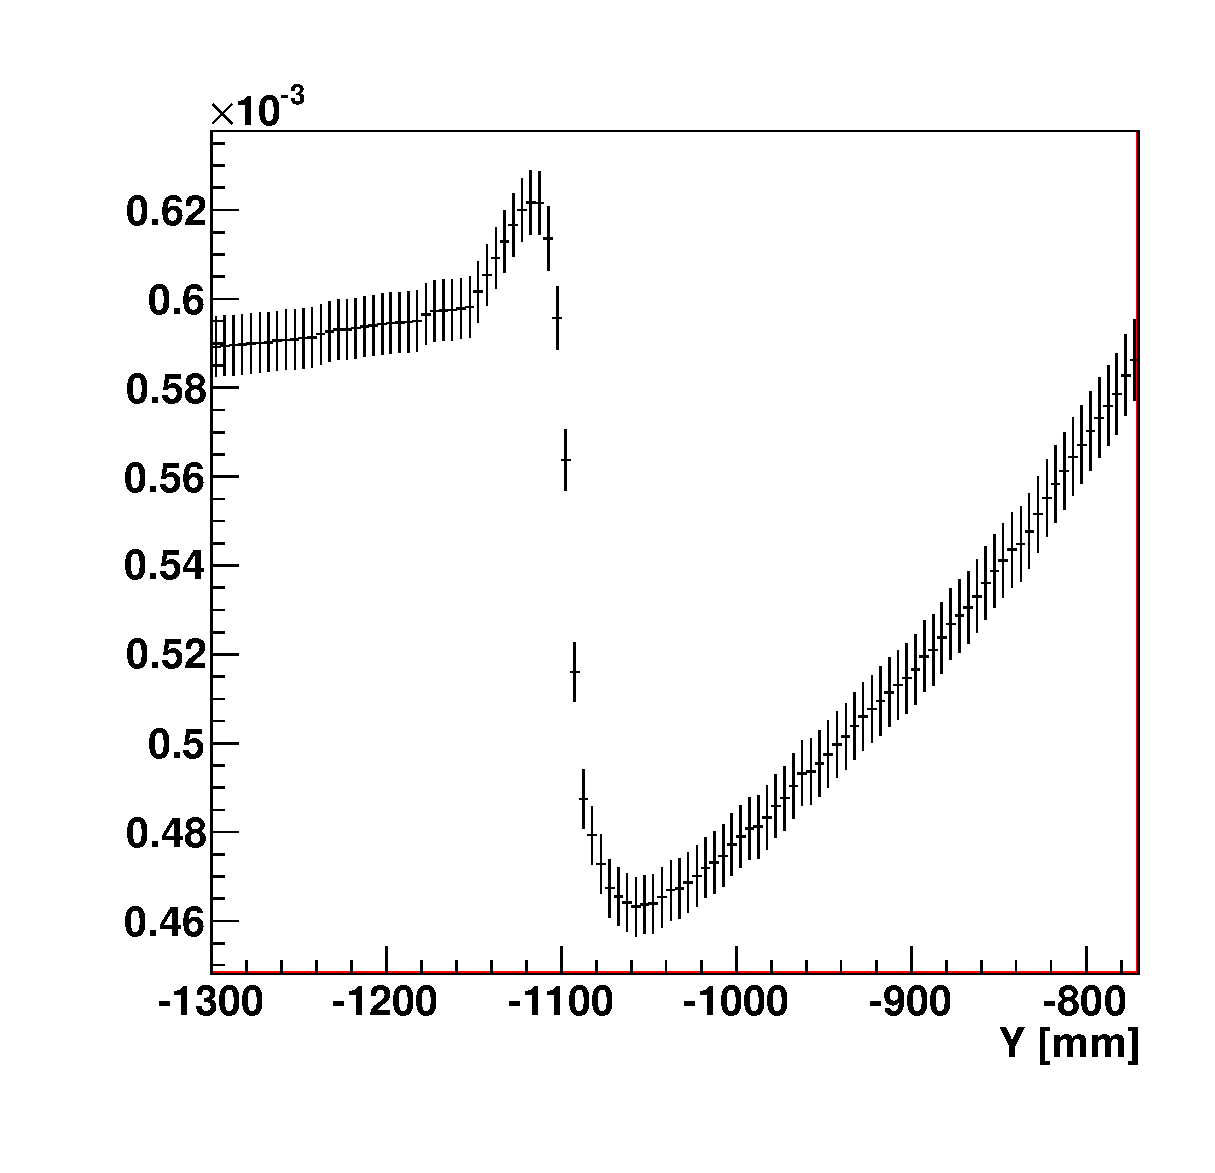
\includegraphics[width=3in]{Figures/FiducialScan-Run1-Yneg.eps}
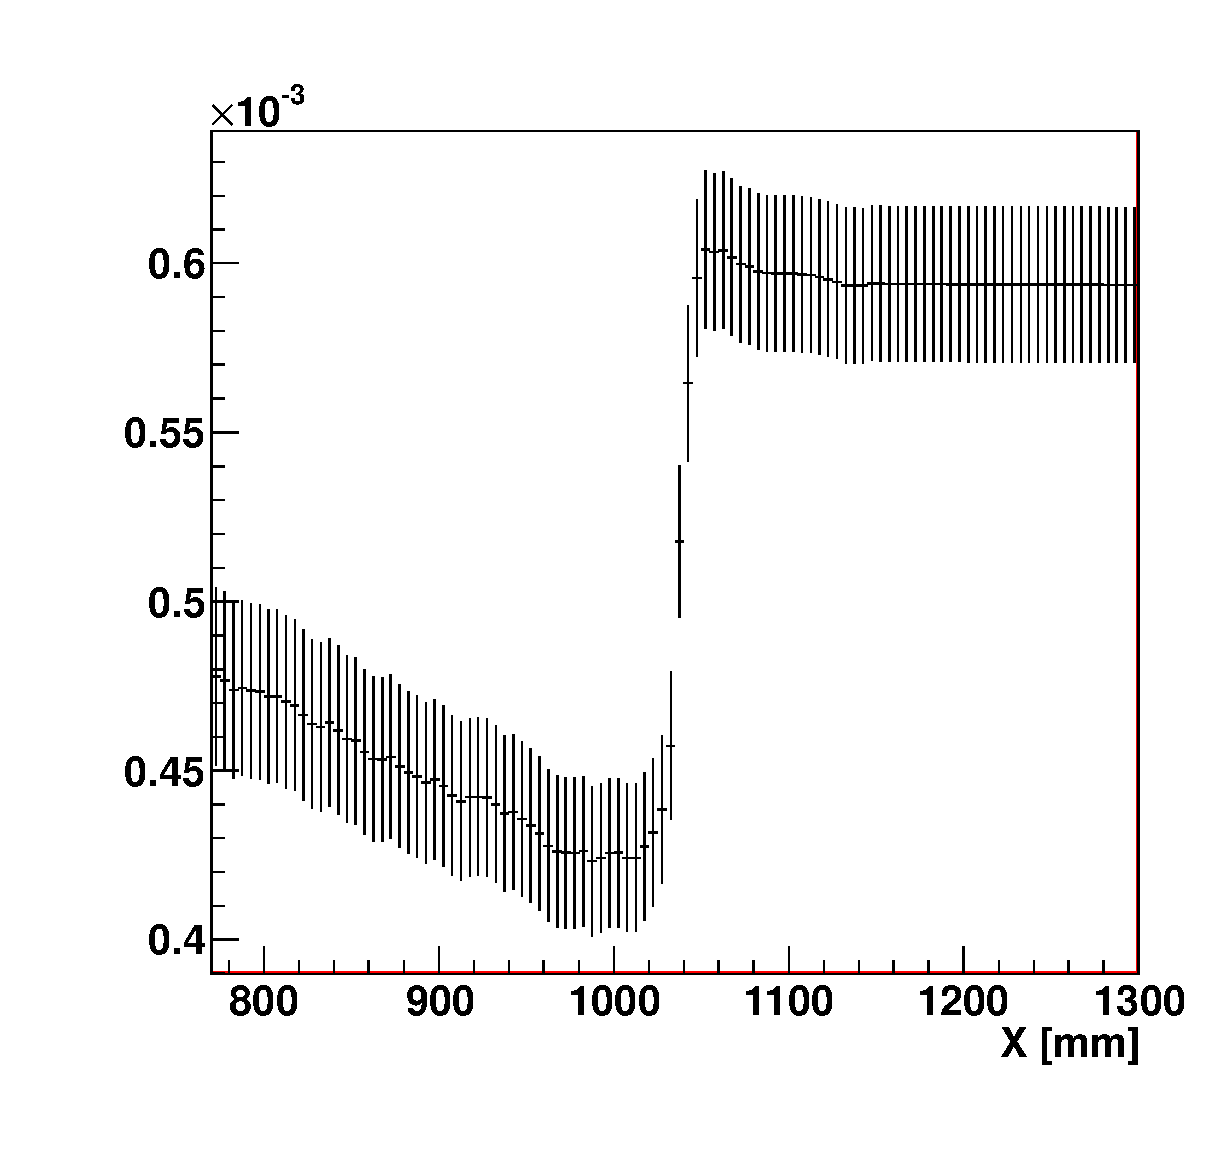
\includegraphics[width=3in]{Figures/FiducialScan-Run2-Xpos.eps}
\caption{Fiducial scan results calculated from 
Eq. \ref{eq:fiducialOptomize} as a function of a given boundary value. 
Left: The fiducial scan results for the negative Y axis boundary of Run 1. 
Right: The fiducial scan results for the positive X axis boundary of Run 2. 
}
\label{fig:fiducialScanResults}
\end{figure}

In practice 
both MC and data samples had the same reconstruction requirements 
of one track per spill that had its start position in the scanned FV. 
This requirement defined $N_{total}$ for both sample types. 
The signal definition was extracted directly from the MC sample 
normalized down by POT to the equivalent data sample. 
The background definition came from the subtraction 
of the MC normalized signal ($N_{s}$) from data $N_{total}$. 
These two definitions were used to calculate 
the value of Eq. (\ref{eq:fiducialOptomize}) for different 
FV boundaries. 
The outputs of these calculations could be used to identify 
the desired minimum values.
Two of the FV scan results are 
shown in Fig. \ref{fig:fiducialScanResults}. 
The figure presents the output results of the negative Y axis scan for Run 1 
and the positive X axis scan for Run 2.  \\

%\begin{figure}[h]
%\centering
%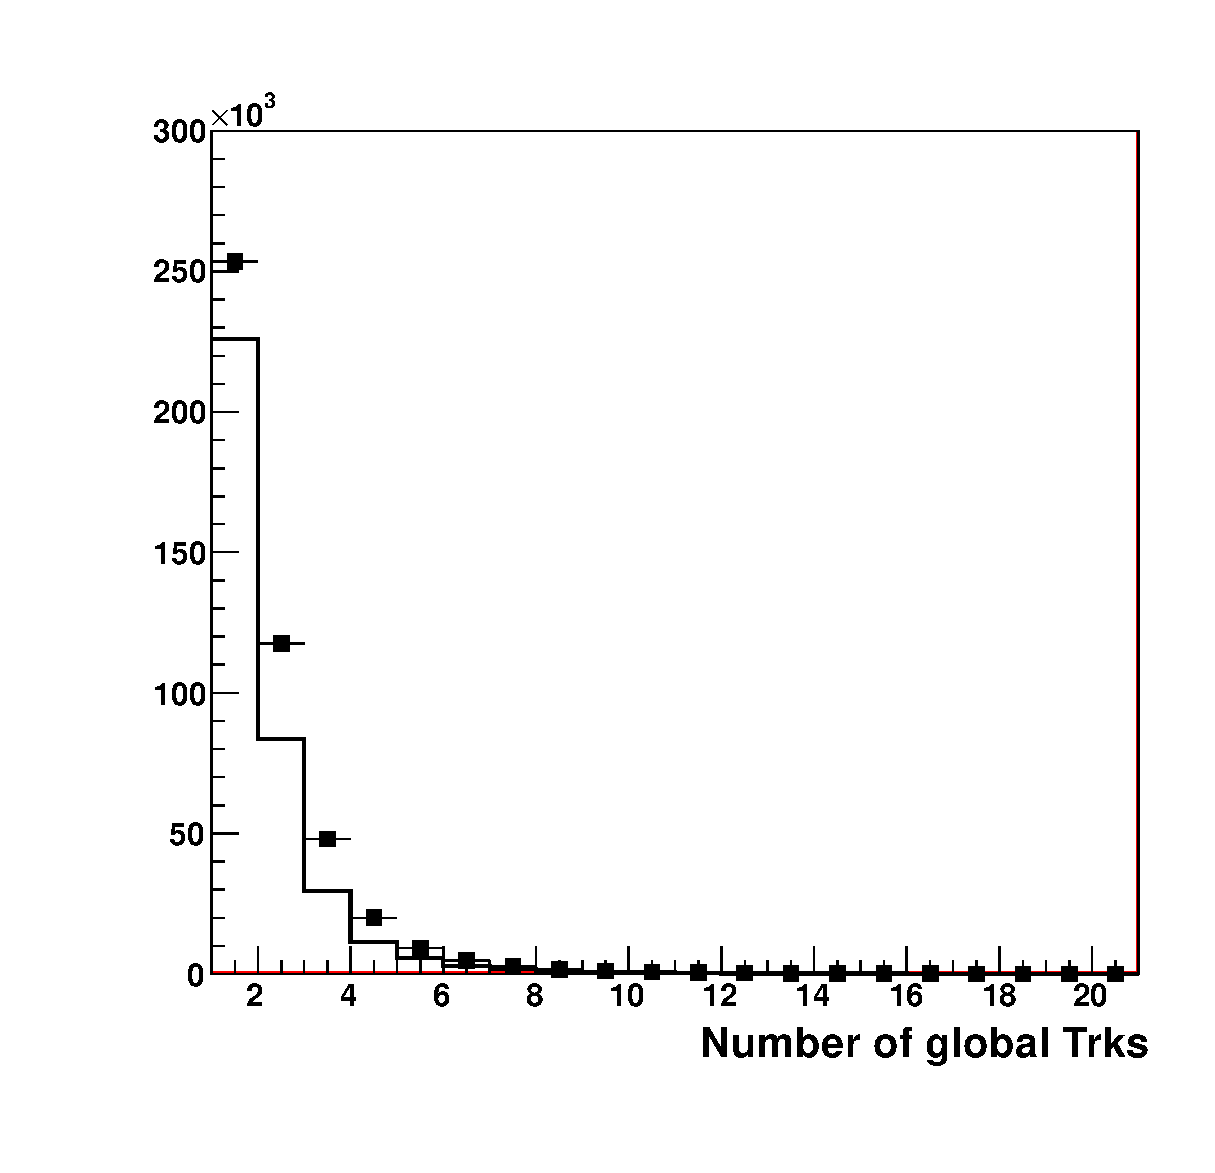
\includegraphics[width=3in]{Figures/triumf-Run1-water-NPIDs.eps}
%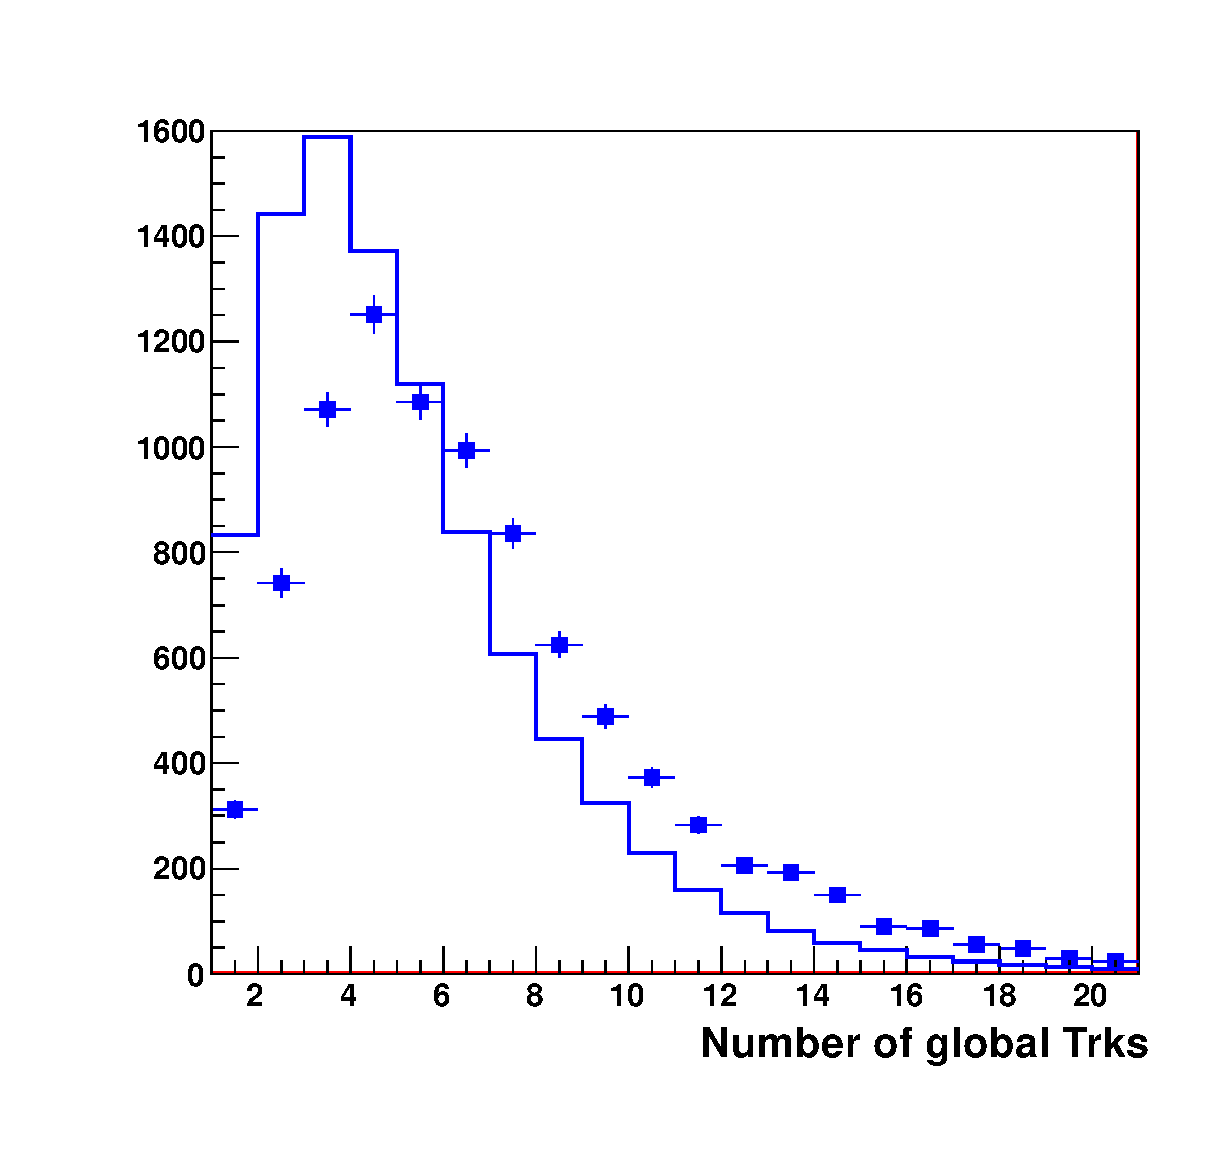
\includegraphics[width=3in]{Figures/triumf-Run2-water-NPIDs.eps}
%\caption{Number of global tracks: Data (points) and MC (Historgam). 
%On the Left (Right) Run 1 (Run2).}
%\label{fig:fiducialNPIDs}
%\end{figure}
\begin{table}
\centering
\begin{tabular}{ccccccc}
%\toprule
 & Run 1 & & & & Run 2 & \\
\cline{1-3}\cline{5-7}\\
Minimum [mm]& Axis & Maximum [mm] & & Minimum [mm]& Axis & Maximum [mm] \\
\cline{1-3}\cline{5-7}\\
-1020 & X & \ \ 990 &\ \ & -1030 & X & \ \ 970 \\
-1045 & Y & \ \ 850 & & -\ 950 & Y & \ \ 850 \\
-3175 & Z & -1010 & & -3175 & Z & -1010 \\
\cline{1-3}\cline{5-7}\\
%\hline\\
%\bottomrule
\end{tabular} 
\caption{The final FV boundaries for the different run periods.}
\label{tab:FV} %FIXME
\end{table}

The final FV boundaries, 
including the restrictions mentioned above, 
are summarized in Table \ref{tab:FV} for both T2K runs. 
A close look at the extracted values reveal that the 
boundaries are not so different between the two runs.

%\subsubsection{Additional checks/tests}
%
%We have issued additional checks on the FV values we extracted 
%with the use of the same sideband samples 
%this was due to possible concerns about \\


%Although we expect the ND280 fiducial cut to remove much of the background
%contribution from magnet interactions and sand muons, we still require a \p0d
%fiducial cut to select \p0d specific interactions. In the X and Y directions, the
%background is a combination of both magnet interactions and sand muons. Whereas
%in the Z direction, we expect a predominantly sand muon background.
%To first order, we have neglected to optimize the \p0d fiducial cut
%for purity and efficiency and instead chosen to cut out regions where a buildup
%of background events is evident. To this purpose, we used a large set of data to
%plot the X, Y and Z positions of the vertex of the highest momentum negative
%track in each event (no fiducial or other cuts were applied here).

%\begin{figure}
%\centering
%\includegraphics[width=5.5in]{Figures/vtxpos.eps}
%\caption{TO BE REMOVED OR REPLACED} 
%\label{fig:figA}%FIXME
%\end{figure}

\subsection{Bunch time windows}

We have studied the  track timing for Run 1 and Run 2
for both data and MC samples.
These studies have revealed a number of points that 
had to be addressed by our bunch time window determination 
and are listed here.
\begin{itemize}
\item
Run 1 has six bunches in each beam spill 
and Run 2 has eight bunches in each beam spill.
\item
Run 2 includes a bunch time shift that was introduced in January 2011.
\item
The MC sample has the same six/eight 
bunch structure as the data sample but the bunches 
are shifted on average by 82-96 ns from the data.
\end{itemize}

\begin{figure}
\centering
%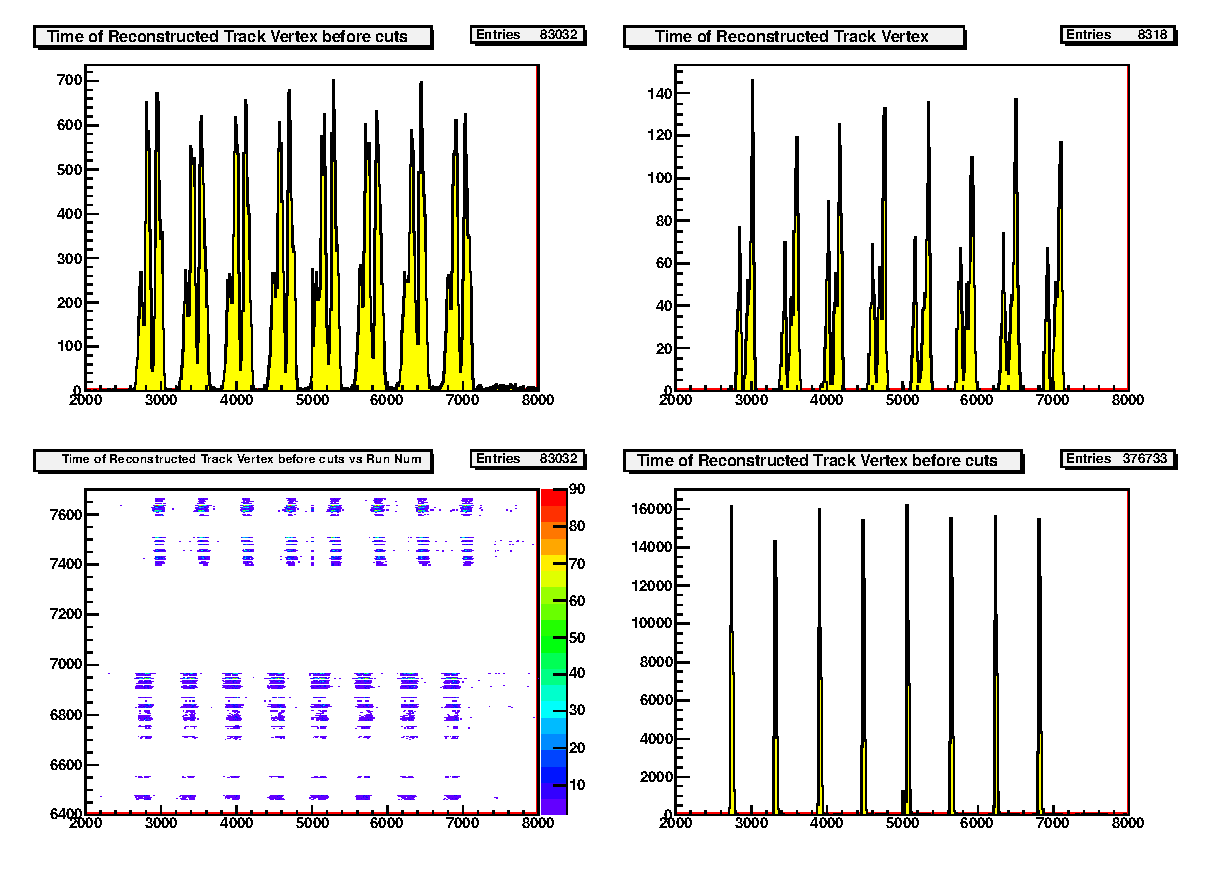
\includegraphics[width=0.95\textwidth]{Figures/BeamStructure.eps}
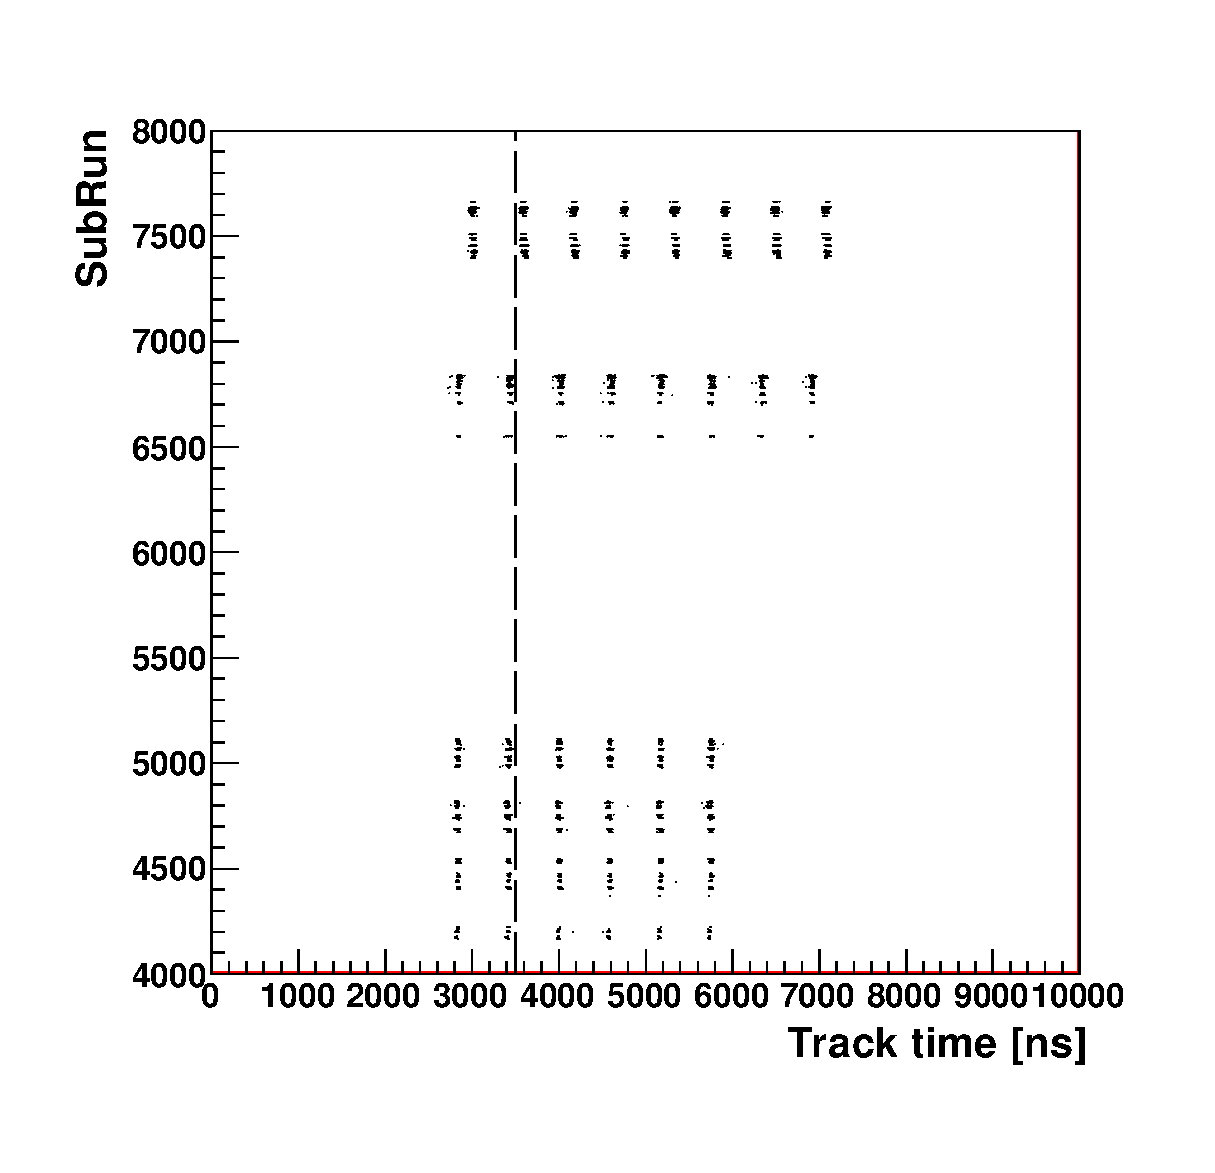
\includegraphics[width=4in]{Figures/spinD-TimeInSpill.eps}
\caption{Track timing as a function of SubRun for the data samples. 
The vertical dash 
line was added to guide the eye on the time shift that was introduced 
in Jan 2011.}
\label{fig:TrackTime}
\end{figure}

In Fig. \ref{fig:TrackTime}, 
which presents the track times 
as a function of their subrun for the data samples, 
one can observe some of these effects. 
A close examination of the figure shows both bunch structures 
and the time shift introduced in Jan 2011. a vertical dash line was added to guide the reader to see this relative shift. \\

%Fitting a gaussian to each of the time peaks, we find the location of the mean
%and determine an acceptable timing window. The same timing windows were used 
%for Run 1 and the two
%different time periods of Run 2. These are given below.

To account for the above conditions, we have decided to define 
the same set of bunch time windows for both runs.  The windows were enlarged to include both the difference between 
data and MC bunch means and the time shift in Run 2. 
Table \ref{tab:BunchTimeWindows} summarizes the 
bunch time windows used in the analyses. 

\begin{table}
\centering
\begin{tabular}{cc}\toprule
Bunch Number & Time window [ns]\\
\hline
 1 & 2700 - 3100\\ 
 2 & 3280 - 3680\\ 
 3 & 3860 - 4260\\ 
 4 & 4440 - 4840\\ 
 5 & 5020 - 5420\\ 
 6 & 5600 - 6000\\ 
 7 & 6180 - 6580\\ 
 8 & 6760 - 7160\\ 
\bottomrule
\end{tabular} 
\caption{The bunch timing windows used in the analysis 
for both Run 1 and Run 2.}
\label{tab:BunchTimeWindows} 
\end{table}


